% Template for Cogsci submission with R Markdown

% Stuff changed from original Markdown PLOS Template
\documentclass[10pt, letterpaper]{article}

\usepackage{cogsci}
\usepackage{pslatex}
\usepackage{float}
\usepackage{caption}

% amsmath package, useful for mathematical formulas
\usepackage{amsmath}

% amssymb package, useful for mathematical symbols
\usepackage{amssymb}

% hyperref package, useful for hyperlinks
\usepackage{hyperref}

% graphicx package, useful for including eps and pdf graphics
% include graphics with the command \includegraphics
\usepackage{graphicx}

% Sweave(-like)
\usepackage{fancyvrb}
\DefineVerbatimEnvironment{Sinput}{Verbatim}{fontshape=sl}
\DefineVerbatimEnvironment{Soutput}{Verbatim}{}
\DefineVerbatimEnvironment{Scode}{Verbatim}{fontshape=sl}
\newenvironment{Schunk}{}{}
\DefineVerbatimEnvironment{Code}{Verbatim}{}
\DefineVerbatimEnvironment{CodeInput}{Verbatim}{fontshape=sl}
\DefineVerbatimEnvironment{CodeOutput}{Verbatim}{}
\newenvironment{CodeChunk}{}{}

% cite package, to clean up citations in the main text. Do not remove.
\usepackage{apacite}

% KM added 1/4/18 to allow control of blind submission


\usepackage{color}

% Use doublespacing - comment out for single spacing
%\usepackage{setspace}
%\doublespacing


% % Text layout
% \topmargin 0.0cm
% \oddsidemargin 0.5cm
% \evensidemargin 0.5cm
% \textwidth 16cm
% \textheight 21cm

\title{Information Distribution Depends on Language-Specific Features}


\author{Josef Klafka \and Daniel Yurovsky \\
        \texttt{\{jklafka, yurovsky\}@uchicago.edu} \\
       Department of Psychology \\ University of Chicago}

\begin{document}

\maketitle

\begin{abstract}
Although languages vary widely in their structure, all are vehicles for
the transmission of information. Consequently, aspects of speakers' word
choice can be understood through models of optimal communication. One
prediction of these models is that speakers should keep the density of
information constant over the duration of an utterance (R. P. Levy \&
Jaeger, 2007). However, different languages have different structural
properties that constrain the space of a speaker's choices
(e.g.~canonical word order). We build on a method developed by Yu, Cong,
Liang, \& Liu (2016) to analyze the word-level entropy curves of natural
language productions across a diverse set of languages and in diverse
written and spoken contexts. We show that languages impose
characteristic constraints on speaker's choices that predict deviations
from Uniform Information Density, and that cross-linguistic variability
in these deviations is predictable in part from syntactic properties of
those languages.

\textbf{Keywords:}
Uniform information density; language structure; corpus analysis
\end{abstract}

Over 7,000 languages are spoken around the modern world (Simons \&
Fenning, 2018). These language vary along many dimensions, but all share
a core goal: communicating information. If speakers and writers of these
languages act near-optimally to achieve their communicative goals,
regularities of use across these diverse languages can be explained by a
rational theory of communication (Anderson, 1991). Information theory, a
mathematical framework developed by Shannon (1948) to describe the
transmission and decoding of signals, has been a unifying approach for
the recent development of theories of communication in human and machine
language processing (Jelinek, 1976; R. P. Levy \& Jaeger, 2007).

These theories model the process of communication as transmission of
information over a noisy channel. The producer begins with an intended
meaning, packages this meaning into language, and then sends the encoded
meaning to their intended receiver over a communicative channel. The
receiver must then decode the producer's intended meaning from the
signal they receive on their end of the channel. The problem is that
this channel is noisy, and sometimes the signal can be corrupted
(e.g.~the producer can misspeak, or the receiver can mishear). In order
to maximize the probability that the correct meaning is transmitted,
these theories predict that producers should choose linguistic messages
that keep the rate of information constant across words. The intuition
is that if the receiver misperceives a word, and that word contains most
of the information in the sentence, then the communication will have
failed. Because producers cannot predict which word a speaker will
mishear, their best strategy is spread the information evenly across all
of the words in a sentence, i.e.~maintain \emph{Uniform Information
Density} (Genzel \& Charniak, 2002; R. P. Levy \& Jaeger, 2007).

The evidence in favor of Uniform Information Density largely been
situation-specific and English-language driven, while the hypothesis
itself has been applied broadly over the past decade. The original
evidence in favor of Uniform Information Density in R. P. Levy \& Jaeger
(2007) finds that the insertion of complementizers (e.g. ``that'') in
relative clauses in English corresponds to where neighboring words have
high information content. Similarly, A. F. Frank \& Jaeger (2008) argues
that contractions in English such as ``you're'' do not occur when
neighboring words are highly informative. Applications of Uniform
Information Density include determining whether linguistic alignment
takes place (Jaeger \& Snider, 2013), Zipfian word length distributions
(Piantadosi, Tily, \& Gibson, 2011), communication efficiency (Mahowald,
Fedorenko, Piantadosi, \& Gibson, 2013), dialogue and turn-taking (Xu \&
Reitter, 2018) and the significance of ambiguity in language
(Piantadosi, Tily, \& Gibson, 2012), among other research.

However, other recent work has contradicted the Uniform Information
Density hypothesis. Similar to the original R. P. Levy \& Jaeger (2007),
Zhan \& Levy (2018) focuses on information distribution at particular
points in sentences. Zhan \& Levy (2018) finds that more
information-rich classifiers in Mandarin Chinese are produced when
production of the neighboring noun is difficult, not when the
information content is high. Jain, Singh, Ranjan, Rajkumar, \& Agarwal
(2018) examine word order across spoken sentences in Hindi, a freer word
order language than English, and find that information density has no
significant effect on determining a Hindi speaker's word order.

Recently, Yu et al. (2016) developed a more direct test of the Uniform
Information Density hypothesis, applying the logic used by Genzel \&
Charniak (2002) to look at the distribution of information \emph{within}
individual sentences. Because people process language
incrementally--using the previous words in a sentence to predict the
words that will come next--the amount of information that a word
contains when seen in isolation should increase over the course of a
sentence (Ferrer-i-Cancho, Debowski, \& Prado Martin, 2013). Analyzing a
large corpus of written English, Yu et al. (2016) find a different
pattern: Unigram entropy increases over the first few words of an
utterance and then remains constant until the final word where it again
jumps up (see top of Figure \ref{fig:read_and_plot_exp1}). Yu et al.
(2016) conclude that the Uniform Information Density hypothesis must not
hold for medial words in a sentence.

We extend and generalize Yu et al. (2016) in three ways: We confirm that
this same pattern is found in English--in written language, and in
conversational speech between adults and between parents and their
children. Thus, this entropy curve is a robust feature of English
linguistic productions. We then examine entropy curves
cross-linguistically, and show that characteristic curves vary across
the world's languages. Finally, we show that this variation is
predictable in part from the structure of individual languages
(i.e.~word order). Taken together, our results suggest a refinement of
the Uniform Information Density hypothesis: speakers may structure their
utterances to optimize information density, but they must do so under
the predictable constraints of their language.

\subsection{Calculating entropy
curves}\label{calculating-entropy-curves}

In all of our studies, we used an adaptation of the by-word entropy
method developed by Yu et al. (2016). Given a text or speech corpus
divided into individual sentences, we partition the corpus by sentence
length in number of words. For each word position \(X\) of sentences of
length \(k\), we define \(w\) as a unique word occurring in position
\(X\). We further define \(p(w)\) as the number of times word \(w\)
occurs in position \(X\), divided by the number of total words that
occur in position \(X\) i.e.~the number of sentences of length \(k\).
This creates a probability distribution over the words occurring in
position \(X\), and computing the Shannon (1948) entropy \(H(X)\) of
this probability distribution gives the positional entropy of position
\(X\) in sentences of length \(k\).

\[H(X) = \sum\limits_w p(w)\log\big(p(w)\big)\]

With this measure, we can compute the unigram entropy at each word
position of sentences of each length within a corpus. The result of this
method can be plotted for each sentence length as an \emph{entropy
curve}, which can be visually compared across sentence lengths to
observe how the unigram entropy changes across absolute positions in
each of the sentences. Genzel \& Charniak (2002) similarly examine a
unigram entropy measure on sentences, and found that entropy at the
sentence level increases linearly with sentence index within a corpus.
Uniform Information Density applies this uniformity of entropy rate in
sentences to all levels of speech (R. P. Levy \& Jaeger, 2007), and so
our method obtained from Yu et al. (2016), which examines text at the
word level, should find a monotonically increasing affine function at
the word level.

The entropy curves capture individual variation across positions in
utterances of the same length. This allows us to directly observe and
judge the amount of variation in words that appear in an individual
position of a sentence. We can directly compare any two positions within
utterances to determine the amount of uncertainty, and therefore
information, on average contained by words within that position of
utterances. This method is thus identical in logic to Genzel \& Charniak
(2002), but within sentences instead of across sentences.

\section{Study 1}\label{study-1}

We began by replicating Yu et al.'s (2016) analysis, computing entropy
curves on the British National Corpus--a collection of predominantly
written English (Clear, 1993). We then applied the same method to the
Switchboard corpus--a collection of spoken English (Godfrey, Holliman,
\& McDaniel, 1992). This allowed us to ask whether the characteristic
function identified by Yu et al. (2016) is a general feature of English,
or instead a function of written language.

\section{Data and Analysis}\label{data-and-analysis}

The British National Corpus consists of predominantly (90\%) written
documents collected in the early 1980s and 1990s across a variety of
genres (scientific articles, newspapers, fiction, etc). It also contains
a small collection of corpora from spoken language. All together, the
British National Corpus contains \(\sim\) 100 million tokens. The
Switchboard corpus is a collection of \(\sim\) 2,400 telephone
conversations between unacquainted adults prompted with subjects of
conversation. Switchboard is the corpus used in Levy and Jaeger's (2007)
original demonstration of the Uniform Information Density Hypothesis.

For each corpus, we computed entropy curves using the method described
above for all sentences from length 4 to 30.

\section{Results}\label{results}

The entropy curves computed in both the British National Corpus and
Switchboard were remarkably consistent both across corpora and across
the range of sentence lengths we analyzed (Figure
\ref{fig:read_and_plot_exp1}). Confirming Yu et al.'s (2016) findings,
we find that the positional entropy at the beginning of sentences is
low, then rises and plateaus for sentence-medial word positions before
dropping slightly in the second-to-last position and rising again for
the sentence-final word.

\begin{CodeChunk}
\begin{figure*}[tb]

{\centering 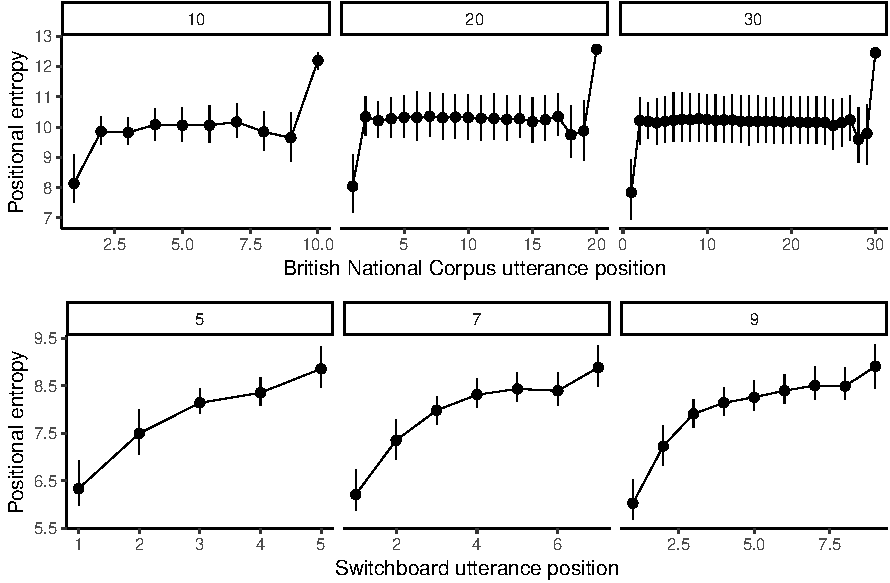
\includegraphics{figs/read_and_plot_exp1-1} 

}

\caption[Representative Entropy Curves for the British National Corpus (top) and Switchboard (bottom)]{Representative Entropy Curves for the British National Corpus (top) and Switchboard (bottom). Points average entropies, error bars show 95\% confidence intervals computed by non-parametric bootstrap.}\label{fig:read_and_plot_exp1}
\end{figure*}
\end{CodeChunk}

The shape of positional entropy curves we find in these two corpora is
notable for two reasons: (1) it does not follow our predictions from
Uniform Information Density, and (2) the distribution is robust across
written and spoken English. This suggests that the entropy curve is
characteristic of the English language. We next asked whether this shape
is a feature even of children's speech, and also whether it varies
cross-linguistically.

\section{Study 2}\label{study-2}

To understand how robust this entropy curve is, we turned to
conversational speech from parent-child interactions. If we find the
same shape even in children's productions, we have even stronger
evidence that the three-step entropy curve is a characteristic feature
of English. We thus used the Child Language Data Exchange System
(CHILDES), a collection of transcripts of parent-child interactions
(MacWhinney, 2014).

\subsection{Data and Analysis}\label{data-and-analysis-1}

We analyzed three separate corpora in CHILDES: The Providence Corpus
(Demuth, Culbertson, \& Alter, 2006), The Shiro corpus (Shiro, 2000),
and the Zhou Dinner Corpus (Li \& Zhou, 2015). The Providence corpus
consists of conversations between six 1--3-year-old American
English-speaking children and their parents recorded in their homes. The
Shiro Corpus consists of prompted Spanish-language narratives
individually collected from over a hundred Venezuelan schoolchildren.
The Zhou Dinner Corpus contains dinner conversations between
5--6-year-old Mandarin-speaking children and their parents collected in
Shanghai. Spanish is an Indo-European language like English, possessing
similar grammar, word order and numerous cognate words to English. In
contrast, Mandarin Chinese is typologically unrelated to English, with
many structural differences between the two languages.

We accessed the transcripts from each corpus using \texttt{childesr}, an
R-interface to a database-formatted version of CHILDES (Sanchez et al.,
in press). We divided all utterances from each transcript into those
produced by the target child, and those produced by all other speakers.
We then applied the same entropy curve method described earlier. For
Mandarin, we used pinyin transliterations of the utterances in the
corpus with demarcated word boundaries. The Chinese characters used for
writing Mandarin do not normally demarcate word boundaries by spacing
words apart, and for normal Chinese writing spaces between word
boundaries are unnatural and such spaces can be difficult to determine
(Bai, Yan, Liversedge, Zang, \& Rayner, 2008).

\subsection{Results}\label{results-1}

\begin{CodeChunk}
\begin{figure*}[tb]

{\centering 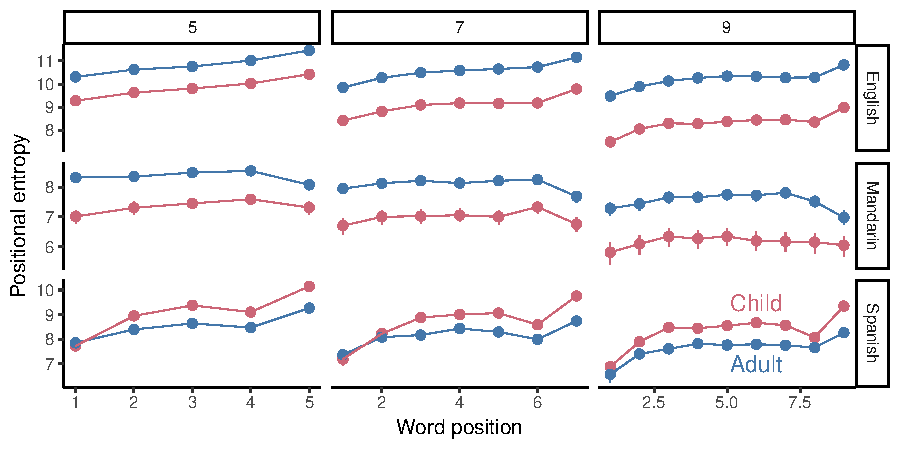
\includegraphics{figs/plot_childes-1} 

}

\caption[Representative Entropy Curves for Three Childes Corpora in English, Mandarin, and Spanish]{Representative Entropy Curves for Three Childes Corpora in English, Mandarin, and Spanish. Points average entropies, error bars show 95\% confidence intervals computed by non-parametric bootstrap.}\label{fig:plot_childes}
\end{figure*}
\end{CodeChunk}

Across corpora, we found similar entropy curve shapes for adults and
children, but distinct shapes for each language. Figure
\ref{fig:plot_childes} shows representative curves across corpora, but
the entropy curve shapes were robust across the full range of utterances
we analyzed. We found a distinct three-step distribution for both the
English and Spanish CHILDES corpora, with a slight dip in the
penultimate position of each sentence. The Mandarin corpus entropy
curve, by comparison, displayed a noticeably lower positional entropy
values in utterance-final positions than in utterance-penultimate
positions.

These results present two important pieces of information. First, the
English Providence corpus entropy curve broadly replicates the curves
found in both the British National Corpus and in Switchboard, our two
previous English corpora. Thus, the entropy curve of English appears not
just in adult-adult conversation, but even in speech produced by parents
to their children, and speech produced by very young children to their
parents. This suggests that it is a highly robust feature of the English
language, as it reflects the structure of even pre-schooled aged
children's speech.

Second, the entropy curves of English, Spanish, and Mandarin were not
identical. No shape resembled the affine function predicted naively from
Uniform Information Density, but also Mandarin was quite different from
both English and Spanish. This suggests that the entropy curve can vary
from language to language. One possibility is that this variation arises
from typological features of language, such as characteristic word
order. We noticed, for instance, a relatively high density of
determiners in the penultimate position of English and Spanish
utterances, which could account their characteristic penultimate dip. In
our final analysis, we explored this possibility directly, analyzing a
large set of Wikipedia corpora from diverse languages, and asking
whether variability in their entropy curves was related to variability
in their syntactic structure.

\section{Study 3}\label{study-3}

In order to understand how entropy curves are related to linguistic
structure, we turned to Wikipedia for a larger and more diverse of set
of languages.

\subsection{Data and Analysis}\label{data-and-analysis-2}

Wikipedia has two primary advantages: (1) Individual language corpora
are generally large, and (2) hundreds of languages are represented. To
understand how variability in entropy curves is related to the structure
of language, we used features from the World Atlas of Language
Structures (WALS, Dryer \& Haspelmath, 2013). WALS is a curated
collection of typological features which analyze and classify the
diversity across the world's languages. However, as the collection
includes contributions from many authors studying a heterogeneous set of
topics and languages, most features are missing for most languages. For
our sample, we sought to balance diversity of languages with coverage in
WALS. We selected \(45\) languages for which eight specific WALS
features were coded (Figure \ref{fig:clust_tree}). Unfortunately, these
features all reflected the order of words in a sentence in each language
(e.g.~whether objects come before verbs, whether adjectives come before
nouns). A consistent set of results across these features would be
consistent with an effect of order on entropy curves, but unfortunately
no other feature types are available for comparison.

We computed entropy curves separately for each language as before. In
order to understand how these curves varied across languages, we
developed a method for compressing the curves into a few representative
values. We noticed that curves tended to vary in predictable utterance
positions: The majority were flat in the middle of utterances, but had
either rising or falling slopes at the beginnings and ends. For each
language, for each utterance length \(k\) we computed 5 slopes: The
change between the 1st and 2nd position, the change between the 2nd and
3rd position, the slope between the 3rd position and the 3rd-to-last
position (\(k-1\)), the slope between the 3rd-to-last and the
2nd-to-last position (\(k-1\)), and the slope between the 2nd-to-last
and final positions. We then averaged these slopes across utterance
lengths within a language to estimate a language-typical signature. We
performed an additional analysis dividing each utterance into fifths
evenly and computing the slopes between these fifths. Results from this
second analysis were qualitatively similar.

\subsection{Results}\label{results-2}

We treated these 5 slopes as a vector, allowing us to compute the
pairwise similarity between languages with cosine--a standard measure of
vector similarity (Landauer \& Dumais, 1997). Intuitively, vectors with
a smaller angle between them are more similar. Figure
\ref{fig:clust_tree} shows a hierarchical clustering of these 5
dimensional vectors, demonstrating that entropy curve similarity appears
to capture typological relatedly, e.g.~Slavic languages are similar to
each-other.

We then asked whether these pairwise similarities were related to
overlap in linguistic features. For each of the 8 WALS features we
measured, we fit a logistic regression predicting whether two languages
would have the same value for that feature from the similarity of their
pairwise entropy curves. Overlap on all 8 features was reliably
predicted by entropy curve similarity (largest \(p = .001\)), with the
amount of variance in feature overlap predicted varying across
predictors \ref{tab:tab_features}. Order of object and verb (\(83A\))
was the strongest predictor, explaining 16.22\% of the variance in
pairwise entropy curve similarity.

\begin{CodeChunk}
\begin{figure}[tb]

{\centering 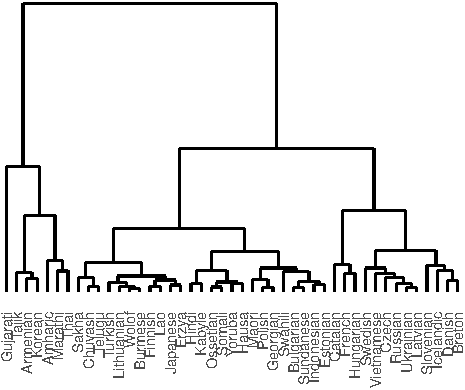
\includegraphics{figs/clust_tree-1} 

}

\caption[A dendrogram estimated from hierarchically clustering the slopes of our 45 languages]{A dendrogram estimated from hierarchically clustering the slopes of our 45 languages}\label{fig:clust_tree}
\end{figure}
\end{CodeChunk}

\begin{table}[tb]
\centering
\begin{tabular}{lrrr}
  \hline
\# & t-value & p-value & r2 \\ 
  \hline
83A & 178.22 & 0.00 & 0.16 \\ 
  95A & 170.98 & 0.00 & 0.15 \\ 
  81A & 153.70 & 0.00 & 0.13 \\ 
  97A & 136.81 & 0.00 & 0.10 \\ 
  144A & 74.43 & 0.00 & 0.03 \\ 
  87A & 39.91 & 0.00 & 0.01 \\ 
  143A & 39.74 & 0.00 & 0.01 \\ 
  82A & 3.23 & 0.00 & 0.00 \\ 
   \hline
\end{tabular}
\caption{Table showing the eight WALS features ranked by significance of effect on the entropy slope cosine distances} 
\label{tab:tab_features}
\end{table}

\section{General Discussion}\label{general-discussion}

Taken together, the results of our studies yield 3 main findings. First,
languages have characteristic entropy curves that can be found in their
productions whether written, spoken, or even spoken by children. These
curves diverge in reliable ways from the affine functions predicted by a
naive Uniform Information Density hypothesis. Second, these
characteristic curves vary across languages--some languages like English
have increasing curves, but others like Mandarin are characterized by
decreasing entropy over the course of an utterance. Finally, these
characteristic curves are related to structural properties of those
languages, for instance their word orders. This work presents an
important rejoinder to models of linguistic productions as optimizing
communicative success. While speakers may structure the information in
their productions to minimize spikes in entropy, speakers operate under
coding models they inherit from their language, and these coding models
constrain the choices they make.

Our work complements the approach of studies such as Aylett \& Turk
(2004), where a language's information distribution is characterized by
a single number representing the average rate of semantic information
transfer per syllable. Each language possesses a characteristic entropy
curve derived from the information distribution within utterances as
well as a measure of the average information expressed by a syllable in
that language.

We expect the characteristic entropy curve for a language to have
important downstream effects for how people process that language. While
conversational turn-taking is universal, there exists cross-linguistic
variation in the average length of time between conversational partners
speaking (Stivers et al., 2009). We predict that one factor in this
variability relates to the shape of a language's entropy curve. A jump
at the end of a language's entropy curve, such as in English, indicates
that there is on average high levels of information at the end of
utterances in that language. Therefore we expect turn-taking times to be
longer in such languages than in languages where there is a drop in the
final segment of the entropy curve, such as Mandarin. We also expect
that readers of a language will take longer on average to read parts of
sentences where the entropy curve is relatively high, due to the
presence of higher information content. This may explain the so-called
wrap-up effect in sentence processing, in which the end of the sentence
in English and other Germanic languages is processed more slowly during
reading (Kuperman, Dambacher, Nuthmann, \& Kliegl, 2010; Stowe, Kaan,
Sabourin, \& Taylor, 2018).

\section{References}\label{references}

\setlength{\parindent}{-0.1in} \setlength{\leftskip}{0.125in} \noindent

\hypertarget{refs}{}
\hypertarget{ref-anderson1991}{}
Anderson, J. R. (1991). The adaptive nature of human categorization.
\emph{Psychological Review}, \emph{98}(3), 409.

\hypertarget{ref-aylett2004}{}
Aylett, M., \& Turk, A. (2004). The smooth signal redundancy hypothesis:
A functional explanation for relationships between redundancy, prosodic
prominence, and duration in spontaneous speech. \emph{Language and
Speech}, \emph{47}(1), 31--56.

\hypertarget{ref-bai2008}{}
Bai, X., Yan, G., Liversedge, S. P., Zang, C., \& Rayner, K. (2008).
Reading spaced and unspaced chinese text: Evidence from eye movements.
\emph{Journal of Experimental Psychology: Human Perception and
Performance}, \emph{34}(5), 1277.

\hypertarget{ref-clear1993}{}
Clear, J. H. (1993). The british national corpus. \emph{The Digital
World}, 163--187.

\hypertarget{ref-demuth2006}{}
Demuth, K., Culbertson, J., \& Alter, J. (2006). Word-minimality,
epenthesis and coda licensing in the early acquisition of english.
\emph{Language and Speech}, \emph{49}(2), 137--173.

\hypertarget{ref-dryer2013}{}
Dryer, M. S., \& Haspelmath, M. (2013). \emph{The world atlas of
language structures online}. Max Planck Institute for Evolutionary
Anthropology.

\hypertarget{ref-ferrer-i-cancho2013}{}
Ferrer-i-Cancho, R., Debowski, L., \& Prado Martin, F. M. del. (2013).
Constant conditional entropy and related hypotheses. \emph{Journal of
Statistical Mechanics: Theory and Experiment}, \emph{2013}(07), L07001.

\hypertarget{ref-frank2008}{}
Frank, A. F., \& Jaeger, T. F. (2008). Speaking rationally: Uniform
information density as an optimal strategy for language production. In
\emph{Proceedings of the annual meeting of the cognitive science
society} (Vol. 30).

\hypertarget{ref-genzel2002}{}
Genzel, D., \& Charniak, E. (2002). Entropy rate constancy in text. In
\emph{Proceedings of the 40th annual meeting on association for
computational linguistics} (pp. 199--206). Association for Computational
Linguistics.

\hypertarget{ref-godfrey1992}{}
Godfrey, J. J., Holliman, E. C., \& McDaniel, J. (1992). SWITCHBOARD:
Telephone speech corpus for research and development. In
\emph{Acoustics, speech, and signal processing, 1992. icassp-92., 1992
ieee international conference on} (Vol. 1, pp. 517--520). IEEE.

\hypertarget{ref-jaeger2013}{}
Jaeger, T. F., \& Snider, N. E. (2013). Alignment as a consequence of
expectation adaptation: Syntactic priming is affected by the prime's
prediction error given both prior and recent experience.
\emph{Cognition}, \emph{127}(1), 57--83.

\hypertarget{ref-jain2018}{}
Jain, A., Singh, V., Ranjan, S., Rajkumar, R., \& Agarwal, S. (2018).
Uniform information density effects on syntactic choice in hindi. In
\emph{Proceedings of the workshop on linguistic complexity and natural
language processing} (pp. 38--48).

\hypertarget{ref-jelinek1976}{}
Jelinek, F. (1976). Continuous speech recognition by statistical
methods. \emph{Proceedings of the IEEE}, \emph{64}(4), 532--556.

\hypertarget{ref-kuperman2010}{}
Kuperman, V., Dambacher, M., Nuthmann, A., \& Kliegl, R. (2010). The
effect of word position on eye-movements in sentence and paragraph
reading. \emph{The Quarterly Journal of Experimental Psychology},
\emph{63}(9), 1838--1857.

\hypertarget{ref-landauer1997}{}
Landauer, T. K., \& Dumais, S. T. (1997). A solution to plato's problem:
The latent semantic analysis theory of acquisition, induction, and
representation of knowledge. \emph{Psychological Review}, \emph{104}(2),
211.

\hypertarget{ref-levy2007}{}
Levy, R. P., \& Jaeger, T. F. (2007). Speakers optimize information
density through syntactic reduction. In \emph{Advances in neural
information processing systems} (pp. 849--856).

\hypertarget{ref-li2015}{}
Li, H., \& Zhou, J. (2015). \emph{Study on dinner table talk of
preschool children family in shanghai} (Master's thesis). East China
Normal University.

\hypertarget{ref-macwhinney2014}{}
MacWhinney, B. (2014). \emph{The childes project: Tools for analyzing
talk, volume ii: The database}. Psychology Press.

\hypertarget{ref-mahowald2013}{}
Mahowald, K., Fedorenko, E., Piantadosi, S. T., \& Gibson, E. (2013).
Info/information theory: Speakers choose shorter words in predictive
contexts. \emph{Cognition}, \emph{126}(2), 313--318.

\hypertarget{ref-piantadosi2011}{}
Piantadosi, S. T., Tily, H., \& Gibson, E. (2011). Word lengths are
optimized for efficient communication. \emph{Proceedings of the National
Academy of Sciences}, \emph{108}(9), 3526--3529.

\hypertarget{ref-piantadosi2012}{}
Piantadosi, S. T., Tily, H., \& Gibson, E. (2012). The communicative
function of ambiguity in language. \emph{Cognition}, \emph{122}(3),
280--291.

\hypertarget{ref-sanchez2019}{}
Sanchez, A., Meylan, S. C., Braginsky, M., MacDonald, K. E., Yurovsky,
D., \& Frank, M. (in press). Childes-db: A flexible and reproducible
interface to the child language data exchange system. \emph{Behavior
Research Methods}. in press.

\hypertarget{ref-shannon1948}{}
Shannon, C. E. (1948). A mathematical theory of communication.
\emph{Bell System Technical Journal}, \emph{27}(3), 379--423.

\hypertarget{ref-shiro2000}{}
Shiro, M. (2000). Diferencias sociales en la construcción del`` yo'' y
del`` otro'': Expresiones evaluativas en la narrativa de niños
caraqueños en edad escolar. In \emph{Lengua, discurso, texto: I simposio
internacional de análisis del discurso} (pp. 1303--1318). Visor.

\hypertarget{ref-simons2018}{}
Simons, G. F., \& Fenning, C. D. (Eds.). (2018). \emph{Ethnologue:
Languages of the world, 21st edition}. Dallas, Texas: SIL International.

\hypertarget{ref-stivers2009universals}{}
Stivers, T., Enfield, N. J., Brown, P., Englert, C., Hayashi, M.,
Heinemann, T., \ldots{} others. (2009). Universals and cultural
variation in turn-taking in conversation. \emph{Proceedings of the
National Academy of Sciences}, pnas--0903616106.

\hypertarget{ref-stowe2018}{}
Stowe, L. A., Kaan, E., Sabourin, L., \& Taylor, R. C. (2018). The
sentence wrap-up dogma. \emph{Cognition}, \emph{176}, 232--247.

\hypertarget{ref-xu2018}{}
Xu, Y., \& Reitter, D. (2018). Information density converges in
dialogue: Towards an information-theoretic model. \emph{Cognition},
\emph{170}, 147--163.

\hypertarget{ref-yu2016}{}
Yu, S., Cong, J., Liang, J., \& Liu, H. (2016). The distribution of
information content in english sentences. \emph{arXiv Preprint
arXiv:1609.07681}.

\hypertarget{ref-zhan2018}{}
Zhan, M., \& Levy, R. (2018). Comparing theories of speaker choice using
a model of classifier production in mandarin chinese. In
\emph{Proceedings of the 2018 conference of the north american chapter
of the association for computational linguistics: Human language
technologies, volume 1 (long papers)} (Vol. 1, pp. 1997--2005).

\bibliographystyle{apacite}


\end{document}
